\documentclass{beamer}
\usepackage[utf8]{inputenc}
\usepackage[T1]{fontenc}
\usepackage{fancyvrb}
\title{Deep Learning Infrastructures}
\date{WASP Deep Learning}
\author[Agents 47]{Group 47}

\usepackage{svg}

\usepackage{graphicx}
\usepackage{caption}
\usepackage{subcaption}

\usepackage{pgfplots}
\pgfplotsset{compat=1.8}
\usepackage{pgfplotstable}
\usepgfplotslibrary{groupplots}

\usetheme{wasp}

\graphicspath{{./graphics/}}

\begin{document}

\begin{frame}
  \titlepage
\end{frame}


\begin{frame}{Infrastructures for Computing}{Introduction}

Different clouds are investigated and compared:
\begin{itemize}
	\item Ericsson Research Cloud (free)
	\item Google Collaborator (free) and Cloud Platform (commercial)
	\item AWS
	\item Microsoft Azure
	\item IBM Bluemix 
\end{itemize}
Mostly of the investigated clouds are commercial  but you can get free trials or be assigned a small amount of credits to explore a limited number of services.   
\end{frame}

\begin{frame}{nfrastructures for Computing}{VMs }

The resources you can get from each clouds service as free tier:
\begin{table}[H]
	\begin{tabular}{|c|c|c|c|}
		\hline
		Infrastructure & No. vCPU&Memory&Storage\\
		\hline
		Ericsson & 4 (Intel Core i7) & 16GB & 40GB\\
		\hline
		IBM Blumix & \multicolumn{3}{c|}{Not applicable for free tier } \\
		\hline
		AWS EC2 & 1 (Intel Xeon)& 1GB& 8GB\\
		\hline
		Azure& 4 (Intel Xeon)& 14GB & 50GB \\
		\hline
		Google Cloud& 4 & 15GB & 40GB SSD\\
		\hline
	\end{tabular}
\end{table}


\end{frame}

\begin{frame}{nfrastructures for Computing}{VMs}

Extra Comments:
\begin{itemize}
	\item Resource of Ericsson VM is preallocated for WASP student account
	\item AWS EC2: Allocation exceeds 10\% of system memory when training a neural network of previous assignment 
	\item Azure and Google Clout Platform would assigned certain amount of credits for new users, the VMs in the table could be kept for approximately 1 month with free credits.
	\item Azure VM for Machine Learning, all packages are pre-installed when a new VM is created, but acceleration could not be afforded by free tiers. 
\end{itemize}

\end{frame}

\begin{frame}{Infrastructures for Computing}{Machine Learning Services}
All the investigated cloud have ML services and compatible with Jupyter notebook. Corresponding service names:
\begin{itemize}
	\item IBM: Watson Studio
	\item AWS: SageMaker
	\item Azure: Machine Learning Workspace
	\item Google: Collaborator
\end{itemize}
Preponderant characteristic of the cloud is that the developer do not concern the resource allocation for the server.  We have several resource options with some of the cloud services but still, very limited for free tiers.
\end{frame}


\begin{frame}{Infrastructures for Computing}{Machine Learning Services}
Computing speed and training results are compare together with local laptop: MacBook Pro, CPU Intel i5, Memory 16GB.
\begin{minipage}[h]{0.48\linewidth}  
	\centering
\begin{figure}[h]
	\centering
	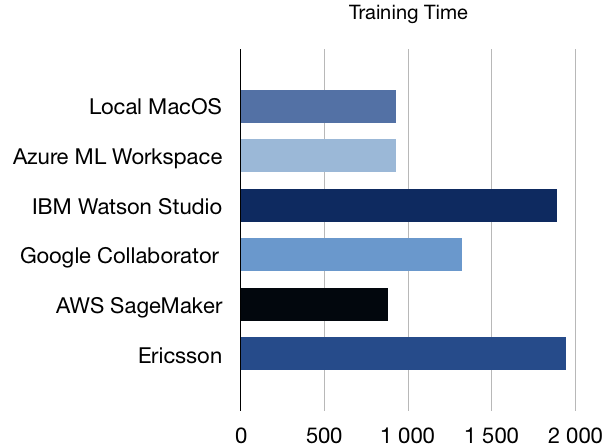
\includegraphics[height=\linewidth]{Training_Time.png}
\end{figure}
\end{minipage}
\end{frame}

\begin{frame}{Infrastructures for Computing}{Machine Learning Services}
\begin{figure}[h]
	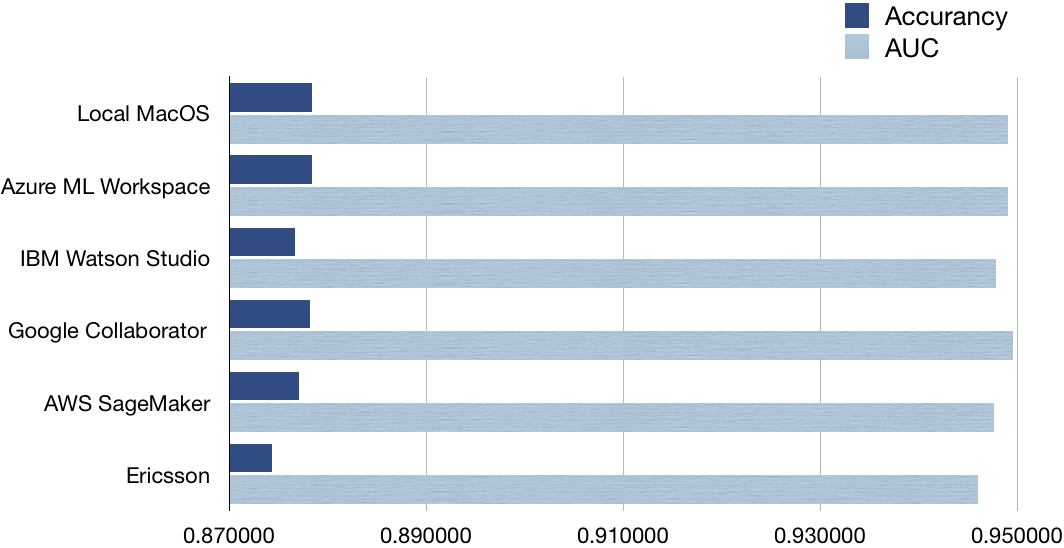
\includegraphics[height=0.5\linewidth]{AA.png}
\end{figure}
\end{frame}

\begin{frame}{Infrastructures for Computing}{Other comments}
\begin{itemize}
	\item Google Collaborator is free for researchers and with GPU/TPU acceleration
	\item Documentations: For most of the clouds the documentations are detailed, especially AWS.  
	\item Setups: Most are  straightforward. User Interface of IBM is not really friendly (to me) and it's not easy to find a right service from the category.
	\item AWS: Most kind of services, clear category, user friendly, easy to setup, etc. Highly recommended if you can afford it.
\end{itemize}
\end{frame}


\bgroup
\setbeamertemplate{background}{}
\setbeamercolor{background canvas}{bg=black}
% \setbeamertemplate{navigation symbols}{}
\begin{frame}[t,plain]{}{}
  \begin{center}
    {\tiny \textcolor{white}{The End}}
  \end{center}
\end{frame}
\egroup

\end{document}
